\subsection{A pre-merge audit}\label{subsec:audit}

Everything in \S\ref{sec:collapse} is computed from the adapter weights, so the
regime of a cohort can be read before any merge is attempted.
Algorithm~\ref{alg:audit} does it. It reads only the $A$ factors: no $B$
factors, no base weights, no forward passes and no data. Its cost is
$O(T^2 r^2 d)$ per layer, about one CPU minute for four rank-$16$ adapters over
eight layers. The thresholds were fixed before any public cohort was measured
and are used unchanged throughout.

\begin{algorithm}[t]
\caption{Pre-merge audit of a LoRA cohort.}
\label{alg:audit}
\begin{algorithmic}[1]
\Require adapters $\{A_t\}_{t=1}^{T}$ on a common base; a sample of layers
  $\mathcal{L}$; thresholds $c_{\mathrm{hi}} = 0.9$, $c_{\mathrm{lo}} = 0.5$
\State $C \gets \emptyset$
\For{each layer $\ell \in \mathcal{L}$}
  \State $V_t \gets \mathrm{orth}\bigl(A_t^{(\ell)\top}\bigr)$ for each $t$
    \Comment{orthonormal basis of the row space}
  \For{each pair $i < j$}
    \State $C \gets C \cup \operatorname{svals}\bigl(V_i^{\top} V_j\bigr)$
      \Comment{cosines of the principal angles}
  \EndFor
\EndFor
\State $\bar c \gets \operatorname{median}(C)$
\State \Return \textsc{collapsed} if $\bar c > c_{\mathrm{hi}}$,
  \textsc{separated} if $\bar c < c_{\mathrm{lo}}$, else \textsc{indeterminate}
\end{algorithmic}
\end{algorithm}

A cohort cannot be repaired by editing its $A$ factors while keeping each
adapter's behaviour. Replacing $A_t$ by $QA_t$ for an invertible $Q$ preserves
the adapter only if $B_t$ becomes $B_tQ^{-1}$, and then the row space, the
principal cosines and $\bar H$ are all unchanged. The geometry is a property of
what the adapters compute, so only retraining or the choice of merge can
change what it does to a merge.

\subsection{Which fine-tuning stacks produce the collapse}\label{subsec:libraries}

Whether two adapters receive the same initial $A$ is decided by library code,
so we read it. In PEFT (version 0.19.1, which wrote all our adapters), the
default initialisation draws $A$ with \texttt{kaiming\_uniform\_} from the
global PyTorch generator; PEFT takes no per-adapter seed and does not reseed.
Two runs therefore receive identical $A$ exactly when the generator is in the
same state as each layer is built: the same seed set beforehand, the same
target modules in the same order at the same rank, and the same device and
data type. Nothing about the task or the data enters.

The question is then what runs before the adapter is created. We read two
widely used fine-tuning stacks at pinned versions. Unsloth~\citep{unsloth2026}
(2026.5.2) gives \texttt{get\_peft\_model} a default \texttt{random\_state} of
$3407$ and sets the seed with it before creating the LoRA layers.
LLaMA-Factory~\citep{zheng2024llamafactory} sets the training seed, $42$ by
default, before the model is loaded. At their defaults both stacks therefore
give every run on one base, target set and rank the same initial $A$: a user
who fine-tunes several tasks without changing the seed obtains a collapsed
cohort. TRL's \texttt{SFTTrainer} builds the PEFT model before it seeds, so its
behaviour depends on the calling script, and we found no seeding before
adapter creation in axolotl. Without any seed the regime does not arise by
accident, since fresh processes start the generator differently. This is a
reading of source code, not a measurement.

\subsection{Prevalence in public adapters}\label{subsec:public}

Our own cohorts say nothing about anyone else's, so we ran the audit on public
cohorts under a protocol registered before any adapter was downloaded. We
walked the HuggingFace model index filtered to PEFT and sorted by downloads,
which weights the sample towards adapters that are used, and grouped adapters
into cohorts by publisher and base model. A cohort entered if it had at least
two readable LoRA adapters of rank at least $4$ on one base, sharing a target
module. Every criterion was checked from metadata before any weight was
fetched, and no cohort was skipped after inspection. We walked $1000$ models to
reach the registered $50$ cohorts; five could not be scored, leaving $45$.

\begin{figure}[pos=tbp]
\centering
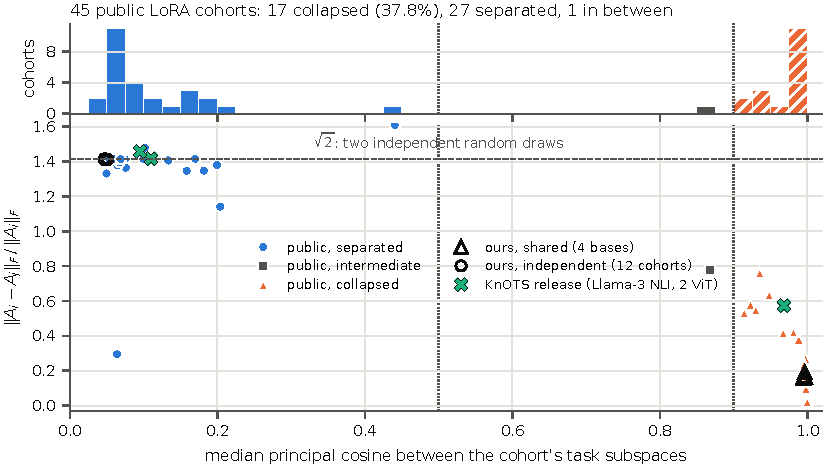
\includegraphics[width=\textwidth]{nc/figures/fig3_prevalence.pdf}
\caption{The $45$ public LoRA cohorts, sampled by a frame registered before
any download. Horizontal axis: median principal cosine between the cohort's
task subspaces, with the audit thresholds dotted and its histogram on top.
Vertical axis: relative distance between the cohorts' $A$ factors, which is
$\sqrt 2$ for two independent random draws. Two cohorts whose members differ in
rank have no distance and appear only in the histogram. Open markers are our
own cohorts; crosses are the three cohorts released with KnOTS, the one merging
paper among $22$ checked that releases LoRA cohorts.}
\label{fig:prevalence}
\end{figure}

Seventeen of the $45$ cohorts, $37.8\%$, are collapsed; the registered
prediction was $20\%$. The distribution is bimodal rather than a continuum cut
by a threshold (Figure~\ref{fig:prevalence}): $27$ cohorts are separated, with
median cosine $0.076$, and only one falls between the thresholds, at $0.868$.
An unplanned check supports the measurement. If two adapters draw $A$
independently and $A$ moves little, then
$\|A_i - A_j\|_F \approx \sqrt2\,\|A_i\|_F$. The separated cohorts give a
median ratio of $1.414$, as independent draws should, while the collapsed
cohorts range from $0.017$, adapters whose $A$ factors agree to within
$1.7\%$, to $0.760$ (Figure~\ref{fig:prevalence}, vertical axis). One separated
cohort sits at only $0.29$, the single point this check does not explain. Our
own cohorts and the three released with KnOTS (below) fall inside the two
public clusters.

The cohorts that merging papers evaluate on are harder to sample. We checked the
$22$ merging papers we cite in order, intending to audit the first two that
release LoRA cohorts; only one does. KnOTS~\citep{stoica2025knots} releases a
Llama-3-8B cohort of six natural-language-inference adapters and two vision
cohorts. Its language cohort is collapsed, at median cosine $0.968$, and its
vision cohorts are separated, at $0.110$ and $0.095$. A released cohort that a
later merging paper uses as its benchmark~\citep{panariello2025core} is
therefore in the collapsed regime. This is a single paper, so we draw no
conclusion about merging benchmarks in general.
